\section{Tradeoff Between Cumulative Probability Mass and Memory in Top-$k$ Truncation}
\label{app:tradeoff}
{Forward KL is defined as an expectation over the teacher's full vocabulary distribution, but computing it over the entire vocabulary incurs substantial memory overhead.
We therefore approximate the forward KL using only the teacher's top-$k$ tokens in \method.
To analyze whether a small $k$ preserves sufficient probability mass, we measure the following for different values of $k$:
(i) the average cumulative probability mass covered by the top-$k$ tokens; and 
(ii) the memory required to store the top-$k$ token probabilities and token indices for each batch.
\autoref{fig:topk_tradeoff} shows the tradeoff between cumulative probability mass and memory usage as $k$ varies.
While memory increases linearly with $k$, the cumulative probability mass quickly saturates.
Empirically, $k=16$ retains most of the probability mass while incurring a relatively small memory overhead of 144\,MiB.
Accordingly, we use $k=16$ in our main experiments.}
\begin{figure}[H]
  \centering
    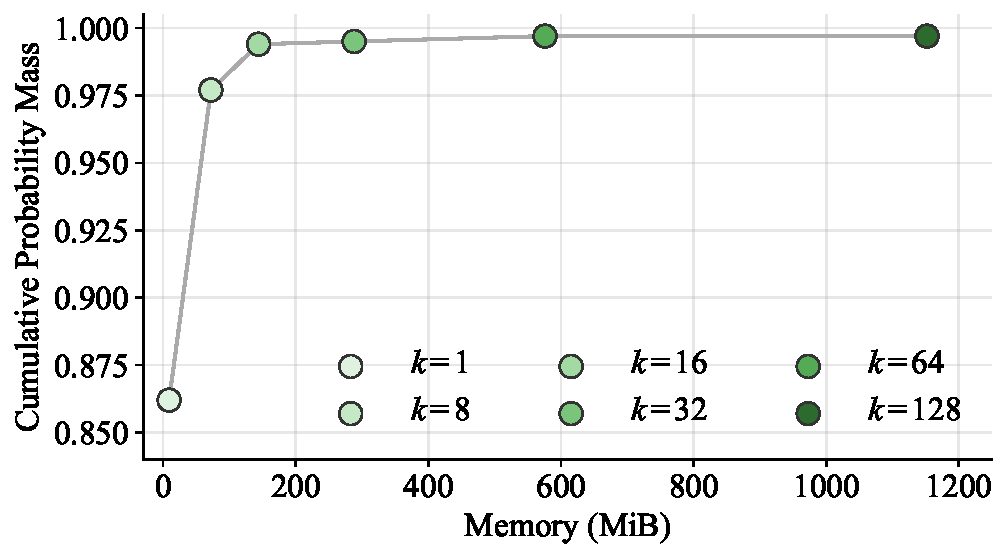
\includegraphics[width=0.5\linewidth]{figure/topk_tradeoff.pdf}
  \caption{Tradeoff between cumulative probability mass and memory usage under top-$k$ truncation. Memory increases linearly with $k$, while the cumulative probability mass quickly saturates.}
  \label{fig:topk_tradeoff}
\end{figure}
